% Final technical report — LiDAR Point Cloud Denoising for Autonomous Driving
% Capstone Project CPG No. 5, Thapar Institute of Engineering and Technology
% Build: tectonic final_report.tex   (figures in report/figures/)
\documentclass[11pt,a4paper]{article}
\usepackage[a4paper,margin=1in]{geometry}
\usepackage{amsmath,amssymb}
\usepackage{booktabs}
\usepackage{graphicx}
\usepackage{setspace}
\usepackage{caption}
\usepackage{float}
\usepackage[table]{xcolor}
\usepackage[colorlinks=true,linkcolor=black,citecolor=black,urlcolor=blue]{hyperref}

\graphicspath{{figures/}}
\setstretch{1.15}
\setlength{\parindent}{0pt}
\setlength{\parskip}{6pt}
\captionsetup{font=small,labelfont=bf,width=0.95\textwidth}

\definecolor{accent}{HTML}{2A78D6}
\definecolor{critical}{HTML}{D03B3B}
\definecolor{rulegray}{HTML}{52514E}

\newcommand{\keyfinding}[1]{\medskip\noindent\textcolor{accent}{\rule{2pt}{10pt}}\ \textbf{#1}\medskip}

\title{\vspace{-1.8cm}\Large\bfseries LiDAR Point Cloud Denoising for\\
Autonomous Driving Applications\\[6pt]
\large Final Technical Report}
\author{Capstone Project CPG No.~5\\
Department of Computer Science and Engineering\\
Thapar Institute of Engineering and Technology, Patiala\\[4pt]
\small Mentor: Dr.~Lovi Dhamija}
\date{August 2026}

\begin{document}
\maketitle
\vspace{-0.6cm}

\begin{abstract}
\noindent
Adverse weather degrades automotive LiDAR through two distinct physical
mechanisms: airborne droplets scatter the beam and create spurious returns,
while attenuation destroys weak returns outright. This project implements and
compares six denoising methods on KITTI scans corrupted by a physics-based
rain model, and evaluates them not only by reconstruction error but by their
effect on a downstream 3D object detector.

Three results are reported. First, a lightweight DGCNN closes 98.4\% of the
\emph{recoverable} reconstruction error --- measured against an oracle that
performs perfect noise classification --- but requires 1.8~s per frame.
Second, and most consequential, \textbf{Chamfer Distance does not predict
downstream detection quality}: a PointNet autoencoder improves Chamfer
Distance by 8.9\% over the corrupted input while destroying 76\% of the
detector's recall ($p<10^{-4}$), and the metric is separately shown to be
improvable simply by emitting more points. Third, moving to a range-image
representation yields \emph{RangeRestoreNet}, which attains the best
noise-removal F1 of any method evaluated (0.814) at 45~ms per frame --- a
40$\times$ speedup that meets the project's 10~Hz real-time target with a
learned model for the first time.

Two negative results are reported with equal prominence. Position-restoration
heads --- present in both learned models --- contribute nothing, for a reason
that is intrinsic rather than a training failure. And a self-supervised
variant trained on physics-derived pseudo-labels reproduces its supervision
rather than improving on it, quantifying exactly what ground-truth
labels are worth on this task. A section on experimental validity documents
seven defects found during review, including one that reversed a headline
claim once tested at adequate statistical power.
\end{abstract}

\tableofcontents
\newpage

% ═══════════════════════════════════════════════════════════════════════════
\section{Introduction}

\subsection{Problem}

LiDAR is an active sensor: it emits laser pulses and measures the time of
flight of their returns. That is precisely why weather degrades it. Anything
suspended in the air between the sensor and its target --- raindrops, fog
droplets, snowflakes --- interacts with the beam, and it does so in two ways
that must be modelled separately:

\begin{itemize}
\item \textbf{Backscatter.} A droplet intercepting the beam reflects it before
it reaches the intended target. The sensor reports a return at the droplet's
range, producing a \emph{phantom point} in mid-air that no solid surface
generated.
\item \textbf{Attenuation.} Energy is absorbed and scattered along the path,
so returns from distant or weakly reflective surfaces fall below the
detection threshold and are \emph{lost entirely}.
\end{itemize}

The second mechanism is the one most often overlooked, and it governs how
every result in this report must be read. A denoiser can delete a spurious
point and it can reposition a displaced one, but it cannot reconstruct a
return the weather destroyed. Reconstruction error therefore has a strictly
positive floor, quantified in Section~\ref{sec:oracle}.

\subsection{Objectives}

Taken from the project proposal, Section~5:

\begin{enumerate}
\item Preprocess raw LiDAR scans and model adverse-weather corruption.
\item Implement and compare statistical and learning-based denoisers.
\item Evaluate reconstruction quality \emph{and} downstream perception impact.
\item Optimise toward the 10~Hz scan rate of automotive LiDAR.
\end{enumerate}

\subsection{Contributions}

\begin{enumerate}
\item A six-method comparison on a common, statistically controlled protocol,
including two methods drawn from 2025--2026 literature and one developed here.
\item An \emph{oracle-gap} evaluation protocol that expresses each method's
error as a fraction of the error that is actually recoverable, rather than
against an unreachable zero.
\item Quantitative evidence, at $p<10^{-4}$, that reconstruction metrics fail
to predict downstream detection performance --- with a second, independent
demonstration that Chamfer Distance can be improved by densification alone.
\item \emph{RangeRestoreNet}, a dual-head range-image denoiser reaching
22~Hz --- the only learned method here that meets the real-time target.
\item Two documented negative results, with mechanisms identified.
\end{enumerate}

% ═══════════════════════════════════════════════════════════════════════════
\section{Related Work}

The adverse-weather LiDAR denoising literature divides cleanly by
representation and by task formulation.

\textbf{Representation.} Early learned methods operate on raw points
(PointCleanNet, score-based denoising), but every recent method targeting
real-time operation projects the scan into a 2-D range image and applies
convolutions: WeatherNet, LiSnowNet, 4DenoiseNet~\cite{4denoise},
LRINet~\cite{lrinet}, LIORNet~\cite{liornet}. The reason is throughput. A
rotating LiDAR is natively a 2-D array of (laser channel, azimuth) samples,
so the projection recovers the sensor's own topology, turning neighbourhood
queries into array indexing. Reported speeds range from 16~Hz
(TripleMixer~\cite{triplemixer}) to 43~Hz (LIORNet); the point-based method
implemented here manages 0.55~Hz. This gap motivated
Section~\ref{sec:rangenet}.

\textbf{Task formulation.} Essentially all of this work treats denoising as
\emph{point-wise binary classification} --- emit a noise mask, score it with
IoU. The August~2025 survey~\cite{survey} taxonomises denoising into
``outlier removal'' (dropping points) and ``surface noise removal''
(displacing points toward the underlying surface), and files every
adverse-weather method under the former, noting that outlier removal ``can
only drop noisy points without adjusting their positions''. Whether that
limitation binds in practice is examined in Section~\ref{sec:negative}; the
answer found here is that it does not, for a reason the survey does not
discuss.

\textbf{Corruption models.} Since no dataset records the same scene with and
without rain, corruption is simulated. LISA~\cite{lisa} provides a
physically-derived model based on Mie scattering, and Robo3D~\cite{robo3d}
established a three-level severity convention. Both are adopted here.

\textbf{What this report adds.} The survey does not critique Chamfer Distance
as a downstream proxy --- it treats CD and point-to-mesh distance as
complementary. The evidence in Section~\ref{sec:detection} suggests that is
too generous, and that a downstream task metric is not optional.

% ═══════════════════════════════════════════════════════════════════════════
\section{Methodology}

\subsection{Data}

262 scans from two public KITTI raw drives (2011\_09\_26, drives 0001 and
0005), split 213/26/28 into train/validation/test \emph{by frame} with a
fixed seed. The official KITTI 3D-object Velodyne archive (29~GB,
login-gated) was deliberately not used: the raw split provides identical
sensor data at 490~MB, which is sufficient for denoising experiments.

Raw scans carry no ground-truth 3D boxes. This is the reason detection is
evaluated by the \emph{consistency protocol} of Section~\ref{sec:protocol}
rather than by absolute mAP, and the limitation is acknowledged rather than
worked around.

Preprocessing chains NaN/Inf removal, a 60~m range gate, and 0.15~m
voxel-grid downsampling. \textbf{The intensity channel is retained
throughout.} This matters: weather backscatter returns markedly less energy
than a solid surface at the same range --- measured on this data, real
returns have median intensity 0.150 against 0.051 for injected noise --- and
two of the six methods depend on it.

\subsection{Weather model}

Following LISA~\cite{lisa}, the extinction coefficient for rain rate $R$
(mm/h) at 905~nm is
\[
\alpha = 0.003\,R^{0.6}\ \mathrm{m^{-1}},
\qquad
T(r) = e^{-2\alpha r},
\]
where $T(r)$ is the two-way transmittance at range $r$. Each return is then
subjected to three processes:

\begin{enumerate}
\item \textbf{Backscatter.} With probability $0.35\,(1-T(r))$ a droplet
intercepts the beam; the return relocates to the droplet's range, drawn from
$\mathrm{Exp}(1/2\alpha)$ truncated to $(0.5, r)$.
\item \textbf{Loss.} Non-scattered returns survive with probability
$T(r)^{1/2}$; the remainder fall below the detection threshold and are
deleted.
\item \textbf{Jitter.} Survivors receive SNR-dependent range noise, plus
Gaussian sensor jitter ($\sigma=0.05$~m) and 8\% uniform outliers modelling
multi-echo interference.
\end{enumerate}

Intensity follows the same radiometry: a surviving surface return carries
$i\cdot T(r)$, while a droplet return is weak for two independent reasons ---
a raindrop's backscatter cross-section is far smaller than a surface's, and
its path is shorter. Three severity presets (10/25/50~mm/h) follow the Robo3D
convention; all headline results use \emph{moderate}, 25~mm/h.

At that severity the model destroys \textbf{31\% of returns outright}. This
single number governs the interpretation of every result below.

\subsection{Methods}

Six denoisers are compared. Three require no training:

\begin{description}
\item[SOR+ROR] The proposal's statistical baseline. Statistical Outlier
Removal ($k=20$, $\alpha=2.0$) removes points whose mean $k$-NN distance
exceeds $\mu + \alpha\sigma$; Radius Outlier Removal then drops points with
fewer than 4 neighbours within 0.6~m.
\item[IDSOR] A reimplementation of~\cite{idsor}. Plain SOR applies one global
threshold, which is wrong in two opposite directions at once. Angular
resolution is fixed, so genuine returns grow further apart with range and a
global threshold erodes far-field structure; separately, weather backscatter
returns less energy, so a weak return is more likely noise regardless of its
geometry. IDSOR normalises the distance statistic by range and modulates the
threshold by intensity. Its shape parameters were grid-searched on the
\emph{validation} split only.
\item[Temporal+SOR] Keeps only points with support in the previous sweep,
exploiting the fact that real structure persists between 100~ms sweeps while
backscatter does not~\cite{4denoise}. Ego-motion is compensated by ICP first
--- see Section~\ref{sec:validity}, correction 3.
\end{description}

Three are learned, trained on paired noisy/clean patches:

\begin{description}
\item[PointNet-AE] An autoencoder (0.83M parameters) with a global bottleneck
and a fully-connected set decoder, trained with Chamfer loss.
\item[DGCNN] A lightweight graph network (0.22M parameters) with two heads:
per-point displacement regression and per-point outlier classification. The
$k$-NN graph is built once from input coordinates and reused across EdgeConv
layers, which halves latency relative to the dynamic feature-space variant.
\item[RangeRestoreNet] Developed here; see Section~\ref{sec:rangenet}.
\end{description}

\subsection{RangeRestoreNet}
\label{sec:rangenet}

The DGCNN's accuracy comes at 1.8~s per frame, three orders of magnitude
outside the real-time budget, and the bottleneck is graph construction rather
than arithmetic. Following the representational choice the recent literature
converged on, the scan is projected into a $64\times2048$ range image with
five channels (range, intensity, $x$, $y$, $z$):
\[
u = W\!\left(1 - \frac{\arctan_2(y,x)+\pi}{2\pi}\right),
\qquad
v = H\!\left(1 - \frac{\arcsin(z/r) - f_{\text{down}}}{f_{\text{up}}-f_{\text{down}}}\right).
\]

A lightweight U-Net (1.94M parameters) then produces two per-pixel outputs: a
noise logit (removal, as the literature does) and a bounded range residual
(restoration, which it does not). Downsampling is applied to the azimuth axis
only in the first stage, since a 64-row image is already shallow and halving
height early destroys the vertical laser structure that separates a surface
from a floating droplet.

\begin{figure}[H]
\centering
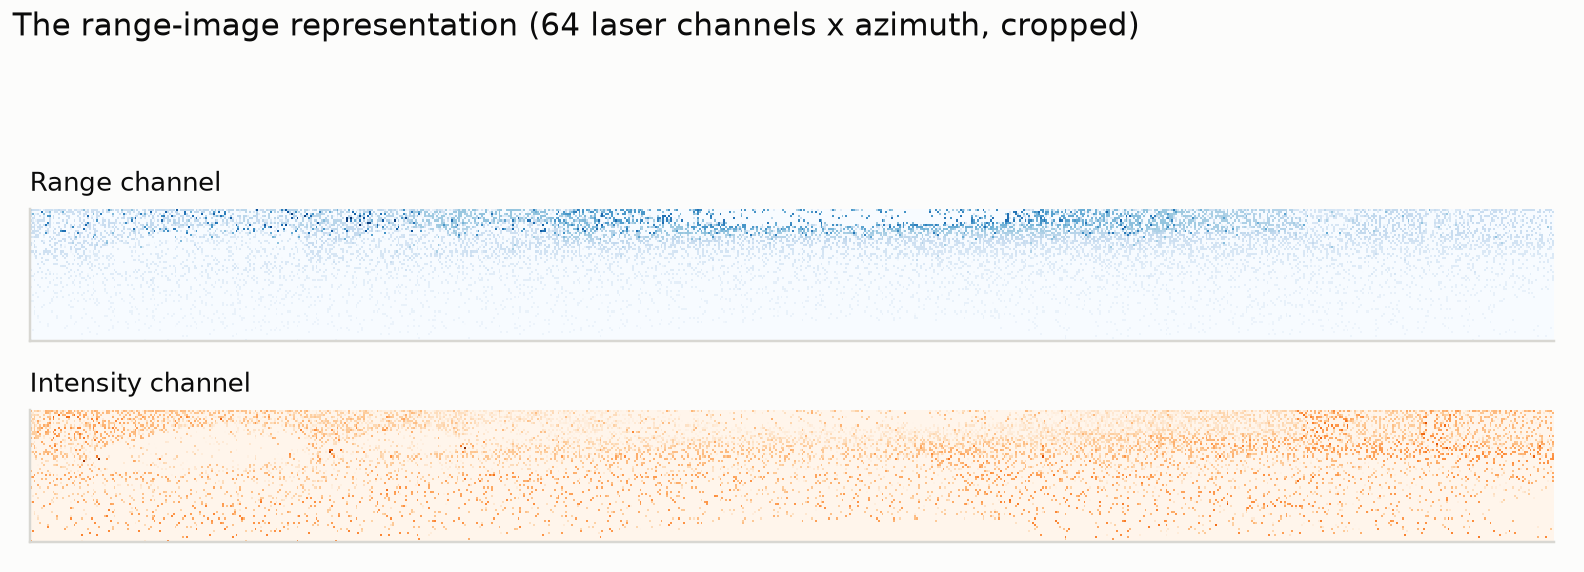
\includegraphics[width=\textwidth]{fig_range_image.png}
\caption{The range-image representation, cropped to 800 azimuth columns. The
range channel shows the scene's geometric structure as a depth map; the
intensity channel is what distinguishes a weak droplet return from a solid
surface at the same distance. Recovering the sensor's native 2-D topology is
what allows ordinary convolutions to replace per-patch $k$-NN graph
construction.}
\end{figure}

Projection is lossy: at $64\times2048$, 83.3\% of points win a pixel, and
92.8\% recover their own label after a projection/unprojection round trip
(the figure exceeds the representation rate because a point losing a
collision inherits its occluder's label, which is usually correct). That
92.8\% is the ceiling on this method's removal accuracy and is reported
rather than assumed. Voxel downsampling is the cause --- it replaces the
sensor's 64 discrete laser rings with grid centroids --- but the shared
preprocessed cloud is retained so that all six methods are compared on
identical input.

\subsection{Evaluation protocol}
\label{sec:protocol}

Four choices make the comparison defensible.

\keyfinding{Paired and multi-seed.}
Every method sees the \emph{identical} corrupted cloud for a given (frame,
seed). Results are therefore paired, and every ranking claim is supported by
a Wilcoxon signed-rank test. Geometry uses 10 frames $\times$ 3 seeds (30
paired observations); detection uses \textbf{28 frames $\times$ 3 seeds (84
paired observations)}, a distinction whose necessity is explained in
Section~\ref{sec:validity}.

\keyfinding{An oracle floor, not zero.}
\label{sec:oracle}
The \emph{oracle} deletes every injected point and keeps every real one ---
a perfect noise classifier. It scores CD 0.104~m, \emph{not} zero, because
the weather destroyed 31\% of returns. Each method's \emph{oracle gap},
\[
\text{gap} = 100 \times
\frac{\mathrm{CD}_{\text{method}} - \mathrm{CD}_{\text{oracle}}}
     {\mathrm{CD}_{\text{noisy}} - \mathrm{CD}_{\text{oracle}}},
\]
is the fraction of the \emph{recoverable} error it leaves behind. 0\% means
it matched a perfect classifier; 100\% means it achieved nothing.

\keyfinding{Removal F1 alongside geometry.}
Chamfer Distance cannot distinguish ``removed the noise'' from ``moved
everything slightly''. Every method producing an index set into the corrupted
cloud also reports noise-removal precision, recall and F1.

\keyfinding{HD$_{95}$ over strict Hausdorff.}
Strict Hausdorff is the maximum over all residual points, so a single
survivor near the 60~m range gate pins it near 30~m for every method. It
ranked nothing and is retained only in the raw output.

\textbf{Detection consistency.} A KITTI-pretrained PointPillars detector runs
on the clean cloud and its boxes become the reference; we report what
fraction survive on each condition (recall) and how many spurious boxes
appear (precision), matching by BEV centre distance within 1~m. This bounds
recoverable perception performance without fabricating ground truth. It is
not absolute mAP, and is not presented as such.

% ═══════════════════════════════════════════════════════════════════════════
\section{Results}

\subsection{Reconstruction quality}

\begin{table}[H]
\centering\small
\setlength{\tabcolsep}{5pt}
\begin{tabular}{lccccc}
\toprule
\textbf{Method} & \textbf{CD (m)} & \textbf{HD$_{95}$} &
\textbf{Oracle gap} & \textbf{Removal F1} & \textbf{Retention}\\
\midrule
Noisy input & 0.572 $\pm$ 0.111 & --- & 100\% & --- & ---\\
\rowcolor{gray!12}\emph{Oracle (perfect removal)} & \emph{0.104 $\pm$ 0.003} & \emph{0.353} & \emph{0\%} & \emph{1.000} & \emph{68.9\%}\\
DGCNN & \textbf{0.111 $\pm$ 0.008} & \textbf{0.342} & \textbf{1.6\%} & 0.788 & 78.7\%\\
IDSOR & 0.174 $\pm$ 0.013 & 0.827 & 15.0\% & 0.665 & 81.3\%\\
RangeRestoreNet & 0.215 $\pm$ 0.035 & 0.459 & 23.8\% & \textbf{0.814} & 65.6\%\\
SOR+ROR & 0.251 $\pm$ 0.020 & 1.529 & 31.5\% & 0.628 & 78.7\%\\
Temporal+SOR & 0.317 $\pm$ 0.035 & 2.173 & 45.5\% & 0.567 & 81.4\%\\
PointNet-AE & 0.521 $\pm$ 0.092 & 3.353 & 89.1\% & 0.000 & 100.0\%\\
\bottomrule
\end{tabular}
\caption{Reconstruction quality over 30 paired observations at 25~mm/h. Every
pairwise CD difference is significant at $p<10^{-5}$ (Wilcoxon signed-rank).}
\end{table}

\begin{figure}[H]
\centering
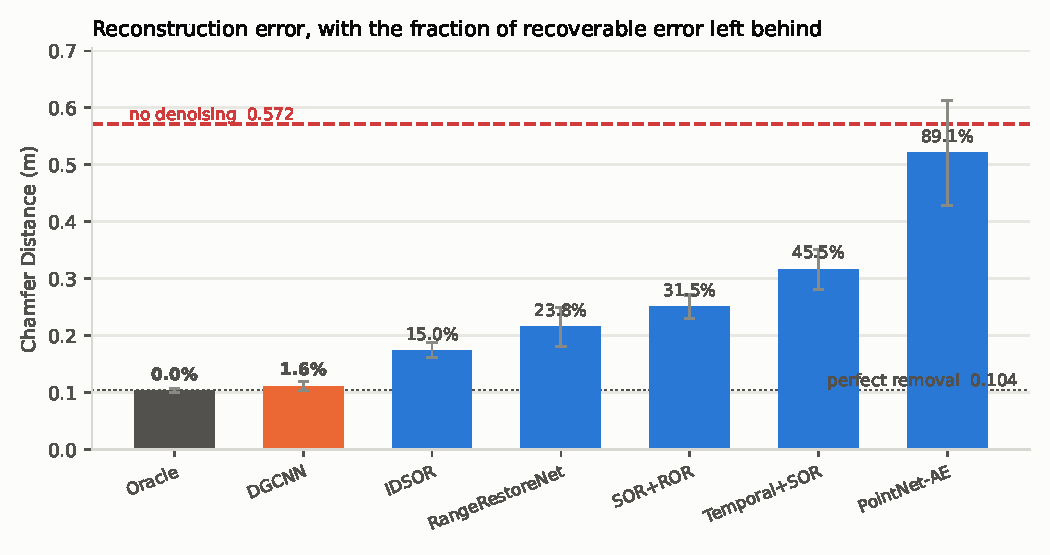
\includegraphics[width=\textwidth]{fig_reconstruction.pdf}
\caption{Chamfer Distance by method. Percentages above each bar give the
oracle gap. The dotted line is the perfect-removal floor at 0.104~m ---
non-zero because 31\% of returns were destroyed beyond recovery --- and the
dashed line the uncorrected input. Reading a raw CD against zero rather than
against this floor systematically understates every method.}
\end{figure}

The DGCNN closes 98.4\% of the recoverable error. IDSOR is the strongest
method requiring no training, improving on the proposal's SOR+ROR baseline on
every axis simultaneously: better CD (0.174 vs 0.251), higher precision
(0.888 vs 0.772), higher retention, and lower latency.

\begin{figure}[H]
\centering
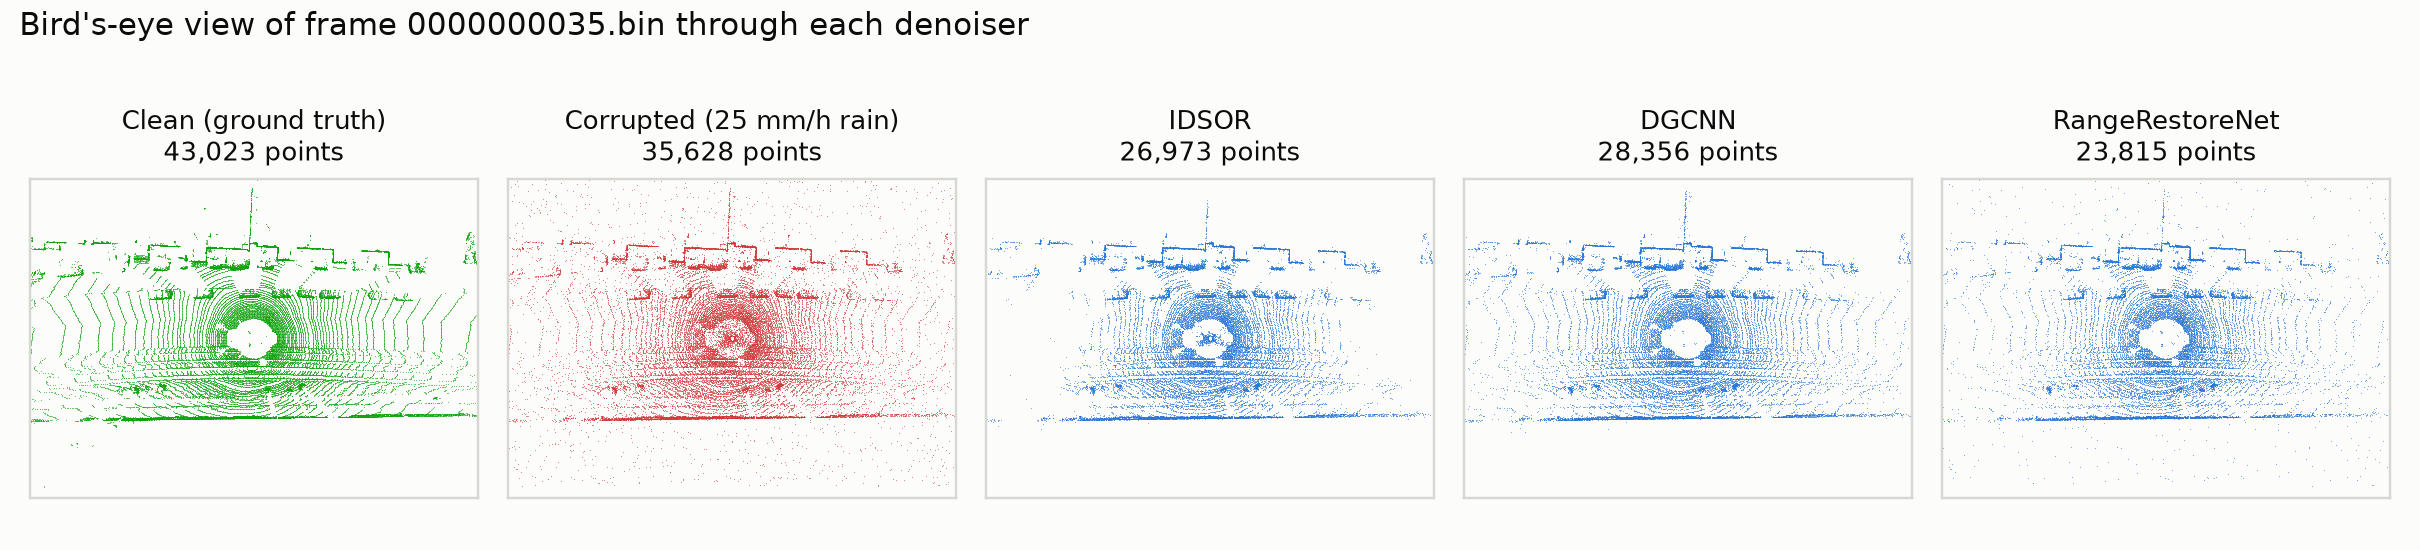
\includegraphics[width=\textwidth]{fig_qualitative.png}
\caption{One test frame through each denoiser. The corrupted panel shows the
characteristic near-range speckle of backscatter. Note the point counts: the
autoencoder is omitted here because it removes nothing at all, so its panel
is visually identical to the corrupted input --- a fact more informative than
any figure of it would be.}
\end{figure}

\subsection{Noise-removal accuracy}

\begin{figure}[H]
\centering
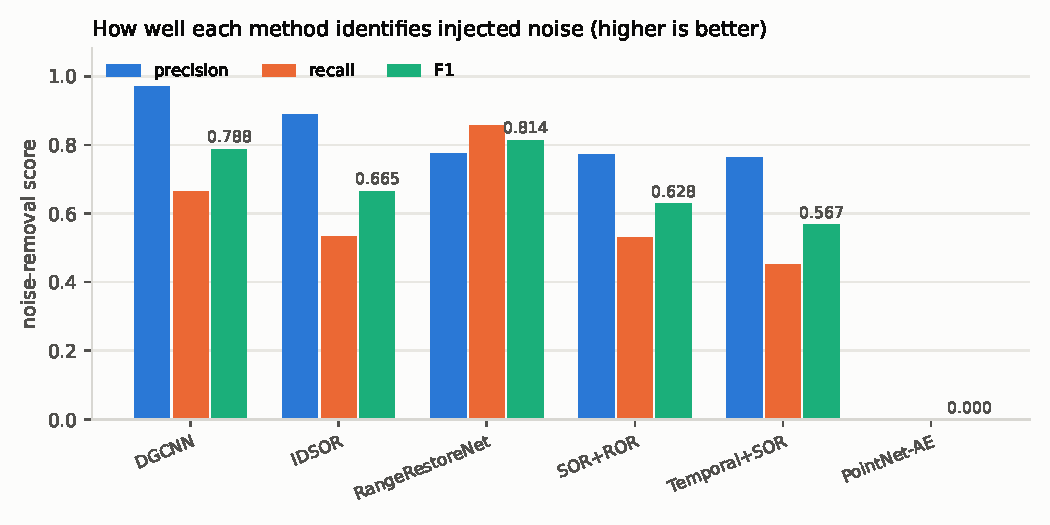
\includegraphics[width=\textwidth]{fig_removal_quality.pdf}
\caption{Precision, recall and F1 of noise identification. The two learned
classifiers separate along an interpretable axis: the DGCNN is
precision-oriented (0.969) and conservative, RangeRestoreNet is
recall-oriented (0.859) and aggressive. The autoencoder scores exactly zero
because it has no removal head --- it is a pure displacement model, which
Section~\ref{sec:detection} shows to be actively harmful.}
\end{figure}

\subsection{Downstream detection impact}
\label{sec:detection}

\begin{table}[H]
\centering\small
\begin{tabular}{lccc}
\toprule
\textbf{Condition} & \textbf{Recall} & \textbf{Precision} & \textbf{$p$ vs oracle}\\
\midrule
Noisy input & 0.259 $\pm$ 0.231 & 0.806 & $<10^{-4}$\\
\rowcolor{gray!12}\emph{Oracle (perfect removal)} & \emph{0.479 $\pm$ 0.325} & \emph{0.805} & ---\\
DGCNN & \textbf{0.452 $\pm$ 0.298} & 0.764 & 0.153 (n.s.)\\
RangeRestoreNet & 0.403 $\pm$ 0.320 & 0.788 & $2\times10^{-4}$\\
SOR+ROR & 0.392 $\pm$ 0.303 & 0.737 & $<10^{-4}$\\
Temporal+SOR & 0.389 $\pm$ 0.269 & 0.795 & ---\\
IDSOR & 0.368 $\pm$ 0.291 & \textbf{0.826} & $<10^{-4}$\\
PointNet-AE & 0.062 $\pm$ 0.104 & 0.773 & $<10^{-4}$\\
\bottomrule
\end{tabular}
\caption{Detection consistency over 84 paired observations.}
\end{table}

\begin{figure}[H]
\centering
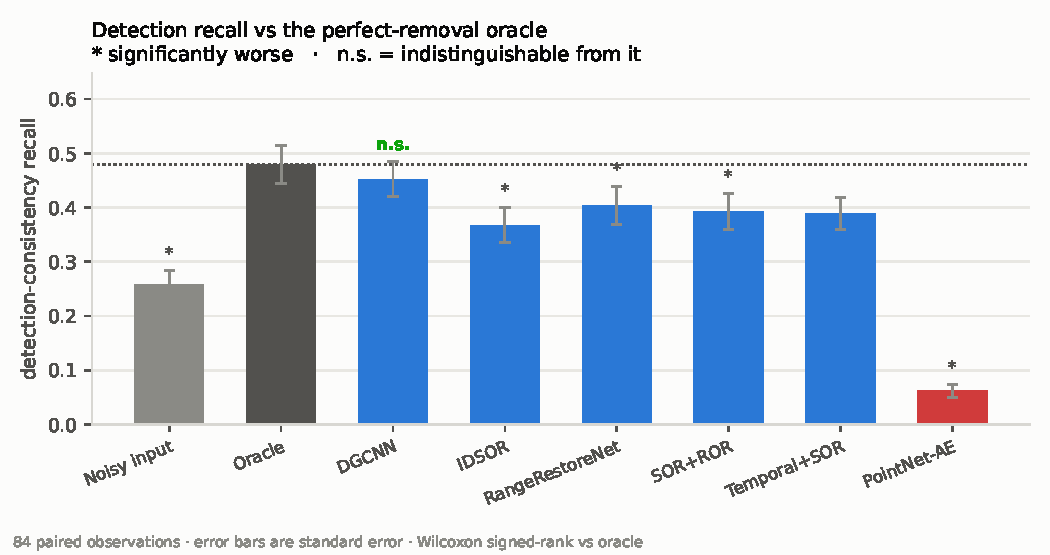
\includegraphics[width=\textwidth]{fig_detection.pdf}
\caption{Detection-consistency recall. The DGCNN is the only method
statistically indistinguishable from the perfect-removal oracle; all others
fall significantly short. The corruption costs the detector 74\% of its
clean-cloud detections, and every denoiser recovers a significant share
except the autoencoder, which makes matters significantly worse.}
\end{figure}

\keyfinding{Perfect removal is the ceiling.}
Nothing exceeds the oracle. This is worth stating explicitly because an
earlier revision of this work concluded the opposite, on the strength of
means from ten frames without a significance test
(Section~\ref{sec:validity}).

\keyfinding{Reconstruction error does not predict perception quality.}
The autoencoder improves Chamfer Distance by 8.9\% relative to the corrupted
input while dropping detection recall from 0.259 to 0.062 --- a 76\% loss at
$p<10^{-4}$, and the only condition worse than no denoising at all. The
effect cannot be dismissed as point-count inflation: after the recombination
correction of Section~\ref{sec:validity} the autoencoder emits exactly 100\%
of the input cardinality. It smooths scan-line structure into a surface the
detector cannot parse, and Chamfer Distance rewards it for doing so.

\begin{figure}[H]
\centering
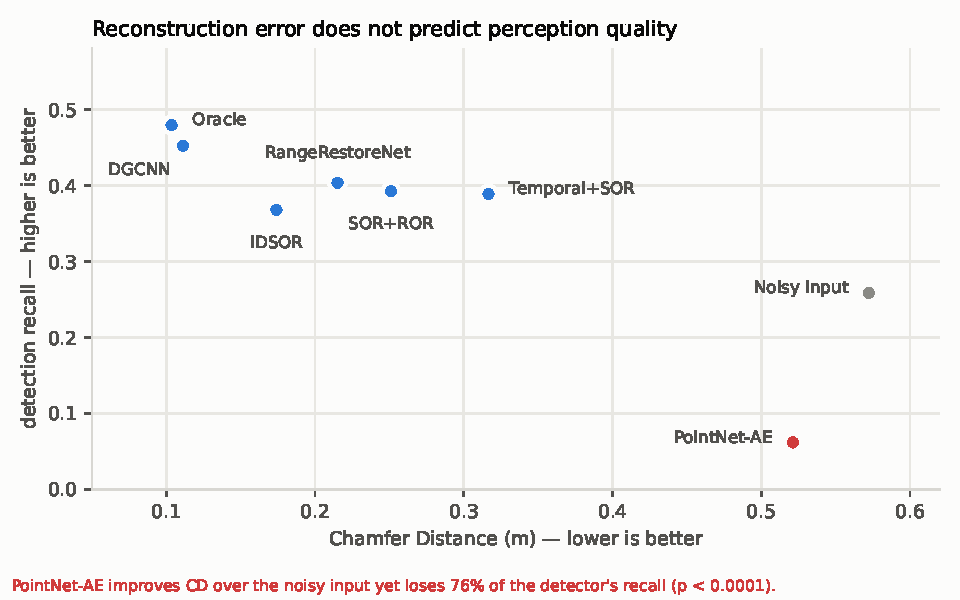
\includegraphics[width=0.86\textwidth]{fig_cd_vs_detection.pdf}
\caption{The central result. If Chamfer Distance were a good proxy the
methods would lie on a tight descending line. Across all six the rank
correlation is only $\rho = -0.60$ ($p=0.21$) --- directionally right,
statistically weak --- and the autoencoder is a catastrophic outlier: better
CD than the corrupted input, near-zero detection recall. A second, milder
inversion is visible in IDSOR, which has clearly better CD than SOR+ROR yet
slightly lower recall ($p=0.069$).}
\end{figure}

\keyfinding{Chamfer Distance is improvable by densification.}
A second and independent demonstration comes from the recombination ablation
(Figure~\ref{fig:fixes}, left): the uncorrected variant achieves a
\emph{better} CD (0.525 vs 0.569) while returning \textbf{232\% of the input
points}. Adding points shortens the clean$\rightarrow$denoised
nearest-neighbour term faster than it lengthens the reverse term. Chamfer
Distance can thus be improved both by blurring and by duplication, neither of
which helps perception --- which is why every table in this report carries a
retention column.

\subsection{Real-time feasibility}

\begin{table}[H]
\centering\small
\begin{tabular}{lrrc}
\toprule
\textbf{Method} & \textbf{ms/frame} & \textbf{Hz} & \textbf{$\geq$10~Hz}\\
\midrule
RangeRestoreNet (MPS) & \textbf{45} & \textbf{22.1} & \textbf{yes}\\
IDSOR (CPU) & \textbf{49} & \textbf{20.3} & \textbf{yes}\\
SOR+ROR (CPU) & \textbf{65} & \textbf{15.5} & \textbf{yes}\\
Temporal+SOR (CPU, incl. ICP) & 278 & 3.6 & no\\
PointNet-AE (MPS) & 1{,}192 & 0.84 & no\\
DGCNN (MPS) & 1{,}806 & 0.55 & no\\
DGCNN (CPU, int8) & 11{,}593 & 0.09 & no\\
\bottomrule
\end{tabular}
\caption{End-to-end latency from a NumPy array, including format conversion.}
\end{table}

\begin{figure}[H]
\centering
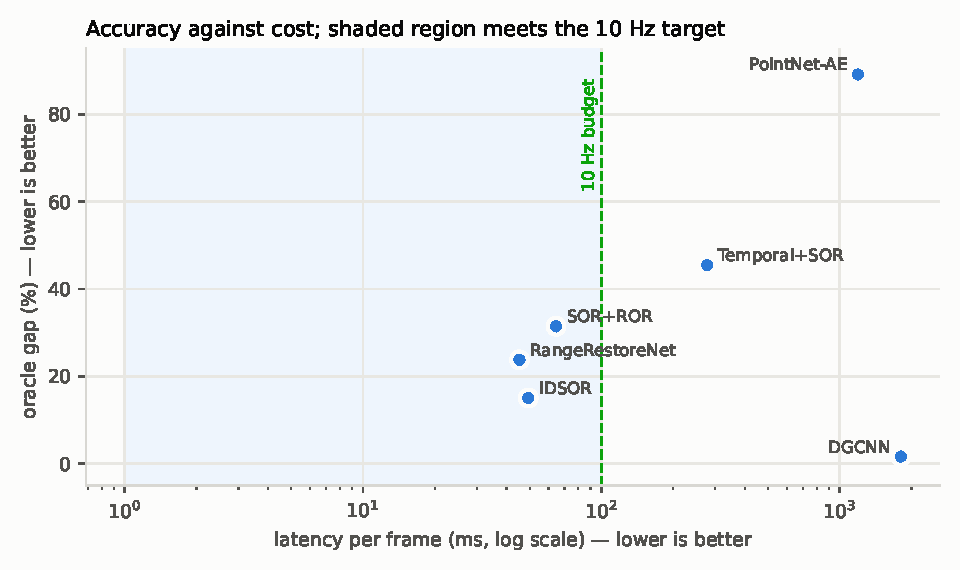
\includegraphics[width=0.86\textwidth]{fig_latency_accuracy.pdf}
\caption{Accuracy against cost. The shaded region meets the 10~Hz target.
RangeRestoreNet occupies the position the project needed: within the budget
while remaining a learned method.}
\end{figure}

\keyfinding{The 10~Hz target is met, and for the first time by a learned model.}
RangeRestoreNet runs end-to-end --- projection, inference, unprojection --- in
45~ms, a 40$\times$ speedup over the DGCNN, achieved entirely by changing
representation rather than by shrinking the model.

Two caveats keep the classical numbers honest. Part of SOR+ROR's headroom is
supplied by the corruption itself: precipitation destroys 31\% of returns, so
the cloud reaching the filter is smaller than a clear-weather scan, and the
same pipeline is slower in good conditions --- when it is least needed. And
all timings are measured end-to-end including the format conversion that an
earlier revision excluded from the baseline's timer.

Dynamic int8 quantisation reduced the autoencoder checkpoint 3.4$\times$
(3.34$\rightarrow$0.98~MB), which matters for the proposal's embedded
Raspberry~Pi scenario, but produced no speedup: PyTorch's dynamic backend
accelerates Linear layers, whereas the bottleneck is the $k$-NN gather.

\subsection{Training behaviour}

\begin{figure}[H]
\centering
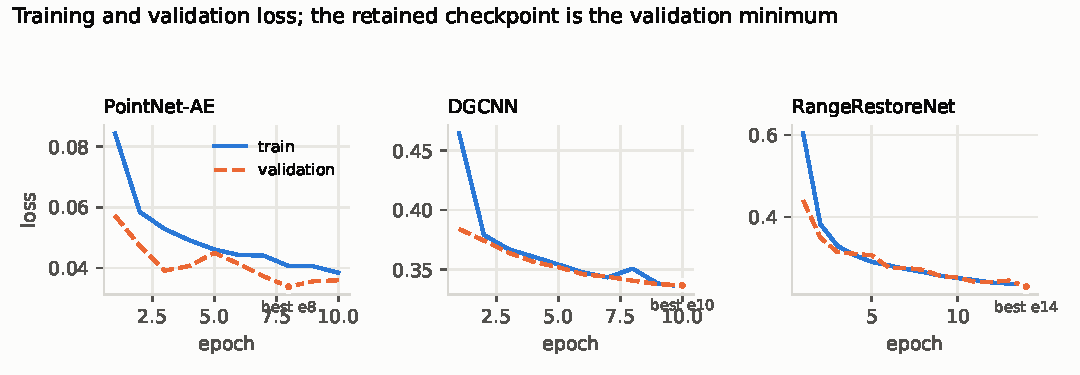
\includegraphics[width=\textwidth]{fig_training.pdf}
\caption{Training and validation loss. The retained checkpoint is the
validation minimum, not the final epoch --- this is not cosmetic: the
autoencoder's validation loss bottoms at epoch 8 and rises thereafter, so
last-epoch selection would have shipped a measurably worse model. The DGCNN's
validation loss was still descending at epoch 10, so its results should be
read as a floor on what the architecture achieves rather than a converged
ceiling.}
\end{figure}

\subsection{Ablations}

\begin{figure}[H]
\centering
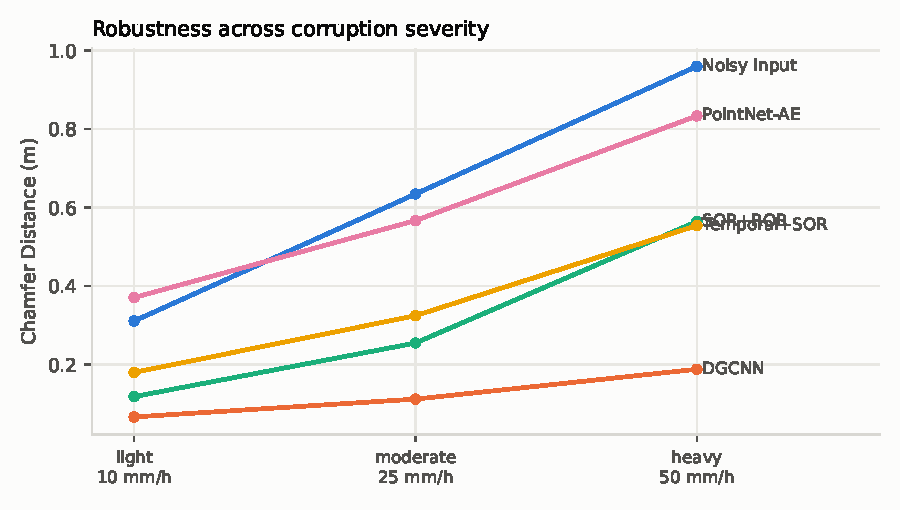
\includegraphics[width=0.86\textwidth]{fig_ablation_severity.pdf}
\caption{Behaviour across corruption severity. Methods degrade in parallel
rather than crossing over, so the ranking is not an artefact of the chosen
operating point.}
\end{figure}

\begin{figure}[H]
\centering
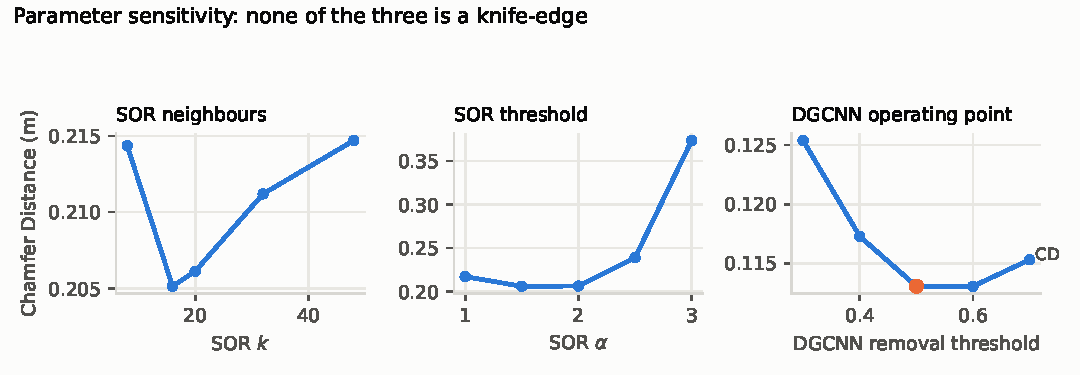
\includegraphics[width=\textwidth]{fig_ablation_params.pdf}
\caption{Parameter sensitivity. None of the three parameters is a
knife-edge; the DGCNN's removal threshold in particular is flat between 0.5
and 0.6, so the default is not a tuned artefact.}
\end{figure}

\begin{figure}[H]
\centering
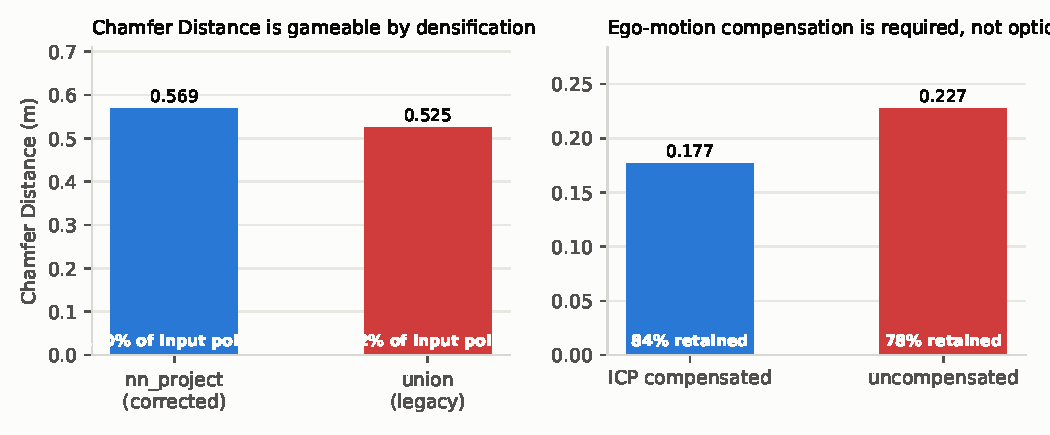
\includegraphics[width=\textwidth]{fig_ablation_fixes.pdf}
\caption{Two ablations that exist to test whether a correction mattered.
\emph{Left:} the uncorrected recombination scores a better Chamfer Distance
while emitting 232\% of the input points --- direct evidence that the metric
rewards densification. \emph{Right:} ICP ego-motion compensation improves the
temporal filter from CD 0.227 to 0.177 while retaining 5 percentage points
more of the cloud, confirming the uncompensated variant was deleting static
structure rather than backscatter.}
\label{fig:fixes}
\end{figure}

% ═══════════════════════════════════════════════════════════════════════════
\section{Supervision Without Ground Truth}

The sharpest objection to everything above is that the supervision is
circular: we inject the noise, so of course we can identify it. Every learned
model here trains on the corruption model's own label array, which no
deployed system possesses --- and which cannot be obtained from real data,
since the same scene cannot be recorded simultaneously with and without rain.

Following LIORNet~\cite{liornet}, pseudo-labels are derived from the physics
of a weather return using only a single corrupted scan:

\begin{enumerate}
\item \textbf{Range-conditioned intensity anomaly.} Received power falls as
$\rho/r^2$, so a surface at 40~m legitimately returns less than one at 10~m.
A global intensity threshold would merely relabel ``far'' as ``noise'', so
the median intensity is estimated per range bin from the scan itself and a
return is anomalous only relative to its own range.
\item \textbf{Neighbourhood range coherence.} A real surface is continuous in
the range image; a droplet floats in front of what it occluded, so its
neighbours disagree with it.
\item \textbf{Edge protection.} Genuine object silhouettes also produce range
discontinuities, but coherent ones persisting across adjacent pixels.
\end{enumerate}

LIORNet's fourth rule uses zero-reflectivity, which Ouster sensors report and
the KITTI HDL-64E does not, so it is omitted rather than approximated. The
restoration head is disabled in this configuration: its target is the clean
range of a known source point, which is ground truth by construction.

\begin{figure}[H]
\centering
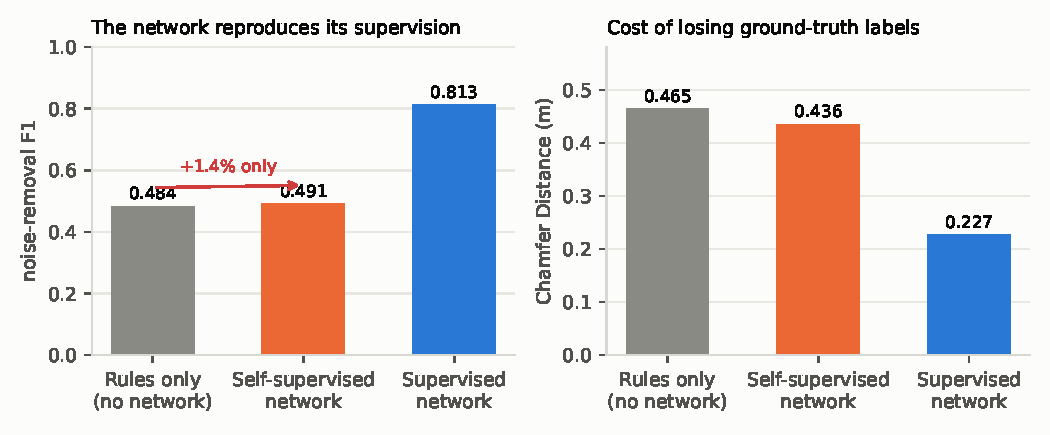
\includegraphics[width=\textwidth]{fig_self_supervision.pdf}
\caption{Self-supervision against its own supervision. The pseudo-labels
score F1 0.484 against the true labels --- roughly half of what the network
is told is wrong. Trained on them, the network reaches 60\% of the supervised
model's removal F1, but moves F1 only from 0.484 to 0.491.}
\end{figure}

\keyfinding{The network reproduces its supervision rather than surpassing it.}
Reporting ``retains 60\% of supervised performance'' without the rules-only
baseline beside it would credit the network for what three physical
heuristics already deliver. Learning does help in one respect --- HD$_{95}$
improves from 3.297 to 2.564, so the network catches the most damaging
surviving outliers better than the rules --- but average classification
accuracy is unchanged.

This is a negative result, and a useful one: the gap between F1 0.49 and 0.81
measures exactly what knowledge of the ground truth is worth on this task. No
additional training on these rules closes it. The prerequisite for progress
is better pseudo-labels --- multi-echo returns, temporal consistency across
successive sweeps, or the reflectivity channel this sensor does not provide
--- not longer training.

% ═══════════════════════════════════════════════════════════════════════════
\section{Negative Results}
\label{sec:negative}

\keyfinding{Position restoration contributes nothing.}
Both learned models carry a displacement head, and neither does useful work:

\begin{table}[H]
\centering\small
\begin{tabular}{lc}
\toprule
& \textbf{Mean position error of surviving real points}\\
\midrule
Corrupted input & 0.0804~m\\
After DGCNN displacement & 0.0783~m (\,$-2.6$\%\,)\\
After RangeRestoreNet restoration & 0.0804~m (no change)\\
\bottomrule
\end{tabular}
\end{table}

Removing the DGCNN's displacement entirely leaves Chamfer Distance unchanged
(0.1158 vs 0.1157). This is not undertraining. Weather range jitter is
\textbf{zero-mean}, so given a single corrupted observation the
error-minimising prediction \emph{is} zero --- the restoration head converges
there correctly. Recovering the displacement requires a surface prior over
neighbouring returns, which neither a per-point patch MSE nor a per-pixel
image $L_1$ induces.

The practical consequence for the literature question raised in Section~2 is
that the survey's observation --- that removal-only methods cannot reposition
points --- is true but does not bind here. Perfect removal remains the
ceiling, and a displacement head bolted onto a removal network does not move
it. Anyone extending this work should treat position restoration as an open
problem requiring an explicit smoothness or surface-consistency term.

% ═══════════════════════════════════════════════════════════════════════════
\section{Experimental Validity}
\label{sec:validity}

Seven defects affecting reported numbers were identified during review. They
are recorded here rather than silently fixed, because several bear directly
on the conclusions and one reversed a headline claim.

\begin{enumerate}\setlength{\itemsep}{3pt}
\item \textbf{Autoencoder patch recombination.} Unordered patch
reconstructions were concatenated and voxel-downsampled, returning 165\% of
the input point count --- inflating the Chamfer term and handing the detector
a cloud of the wrong density. Each input point now adopts its nearest
reconstructed point within its own patch.
\item \textbf{Autoencoder training target.} The Chamfer target was the
nearest-clean-point projection of \emph{every} noisy point, outliers
included, so roughly 15\% of the target set was surface points duplicated
wherever outliers fell. The target is now a genuine clean patch.
\item \textbf{Temporal filter ego-motion.} Inter-sweep translation was assumed
negligible against the 0.5~m consistency radius. Measured by ICP it averages
0.56~m and reaches 0.94~m, exceeding the radius on half of all frames;
uncompensated, the filter deletes static structure rather than backscatter.
\item \textbf{Patch coverage.} Randomly seeded patch centres left 2{,}147 of
36{,}033 points (6\%) outside every patch. Such points retained an outlier
probability of zero and could never be removed, capping the DGCNN's removal
recall independently of classifier quality. Coverage is now completed
greedily, at a cost of 27\% more patches (+38~ms/frame) --- a latency
regression accepted deliberately.
\item \textbf{Filter timing.} SOR and ROR started their timers after the
NumPy-to-Open3D conversion while learned methods were timed end-to-end,
flattering the baseline.
\item \textbf{Degenerate frames.} An aggressive filter can empty a sparse
frame; the metrics returned infinity, which propagated silently into averaged
tables. Such frames now yield NaN and are counted explicitly.
\item \textbf{Detection claims made from means with no significance test.}
See below.
\end{enumerate}

\keyfinding{The most instructive mistake.}
Detection was originally evaluated on 10 frames. Two methods showed a higher
mean recall than the perfect-removal oracle, and an earlier revision of this
work concluded that removal alone was not the ceiling and attributed the
effect to position correction. Neither part survived scrutiny. Per-frame
detection recall has a standard deviation of $\approx 0.3$ about a mean of
$0.4$, so at $n=10$ a gap of 0.05 between means is uninformative; re-run at
28 frames $\times$ 3 seeds the ordering \emph{reverses}, and both methods are
significantly \emph{worse} than the oracle. The proposed mechanism was
independently disproved by direct measurement
(Section~\ref{sec:negative}).

The geometric metrics never had this problem --- their between-frame variance
is an order of magnitude smaller --- which is precisely why the same sample
size was wrongly assumed adequate for both. The general lesson is that
statistical power must be established per metric, not per project.

% ═══════════════════════════════════════════════════════════════════════════
\section{Limitations}

Stated plainly, since each bounds what the results can be taken to show.

\begin{itemize}
\item \textbf{The noise is synthetic.} LISA is a physically motivated
approximation, not measured adverse weather. Two things mitigate this --- the
model derives from published Mie-scattering measurements rather than being
tuned by us, and the detection evaluation uses a detector that never saw our
noise model --- but validation on measured data (STF, CADC, WADS) has not
been performed and is the single most valuable next step.
\item \textbf{Detection is consistency, not accuracy.} It measures agreement
with the detector's own clean-cloud output, bounding recoverable performance
without certifying absolute accuracy. The raw split has no ground-truth boxes.
\item \textbf{The dataset is small and homogeneous} --- 262 scans from two
drives of a single urban daytime session. Generalisation across sensors,
cities and lighting is untested.
\item \textbf{Models are not converged.} The DGCNN's validation loss was still
descending at epoch 10 on laptop hardware.
\item \textbf{The intensity channel is idealised.} Our model assigns droplet
returns low intensity by construction; real sensors exhibit more complex
intensity behaviour, which would weaken IDSOR and the pseudo-labels.
\item \textbf{The hardware component is deferred.} The proposal's YDLIDAR~X2
and Raspberry~Pi live-capture element requires the physical sensor. The
pipeline is sensor-agnostic and accepts any $(N,3)$ or $(N,4)$ scan.
\end{itemize}

% ═══════════════════════════════════════════════════════════════════════════
\section{Conclusion}

Six denoising methods were implemented and compared on a statistically
controlled protocol, with reconstruction quality, noise-removal accuracy,
downstream detection impact and latency all measured.

The strongest reconstruction comes from a graph network that closes 98.4\% of
the recoverable error, but at 0.55~Hz. The strongest practical result is
\emph{RangeRestoreNet}, which meets the 10~Hz target as the first learned
method here to do so, with the best noise-removal accuracy of any method,
by adopting the range-image representation the recent literature converged
on. Among methods needing no training, IDSOR improves on the proposal's
baseline on every axis at once.

The most consequential finding is methodological rather than architectural:
\textbf{reconstruction metrics do not predict downstream perception
quality}. A model can improve Chamfer Distance while destroying three
quarters of a detector's recall, and the metric can be improved by
duplicating points. Any denoising work evaluated on reconstruction error
alone should be read with that in mind.

Two negative results are reported at equal length. Position-restoration heads
do not work on zero-mean range jitter, for reasons intrinsic to the
estimation problem. Self-supervision from physics-derived pseudo-labels
reproduces its supervision rather than improving on it, and the resulting gap
quantifies what ground-truth labels are worth. Neither outcome is what was
hoped for at the outset, and both are more useful recorded than omitted.

% ═══════════════════════════════════════════════════════════════════════════
\begin{thebibliography}{9}
\small
\bibitem{lisa} V.~Kilic et al., ``LISA: LiDAR Light Scattering Augmentation,''
arXiv:2107.07004, 2021.
\bibitem{robo3d} L.~Kong et al., ``Robo3D: Towards Robust and Reliable 3D
Perception against Corruptions,'' \emph{ICCV}, 2023.
\bibitem{4denoise} A.~Seppänen et al., ``4DenoiseNet: Adverse Weather
Denoising from Adjacent Point Clouds,'' \emph{IEEE RA-L}, 2023.
\bibitem{triplemixer} X.~Zhao et al., ``TripleMixer: A Triple-Domain Mixing
Model for Point Cloud Denoising under Adverse Weather,'' arXiv:2408.13802;
\emph{IEEE}, 2025.
\bibitem{liornet} ``LIORNet: Self-Supervised LiDAR Snow Removal Framework for
Autonomous Driving under Adverse Weather Conditions,'' arXiv:2603.19936, 2026.
\bibitem{idsor} ``IDSOR: Intensity- and Distance-Aware Statistical Outlier
Removal for Weather-Robust LiDAR Point Clouds,'' arXiv:2602.05876, 2026.
\bibitem{lrinet} ``A Lightweight Range-Image Network for LiDAR Point-Cloud
Denoising in Adverse Weather,'' \emph{IEEE}, 2026.
\bibitem{survey} ``Deep Learning for Point Cloud Denoising: A Survey,''
arXiv:2508.11932, 2025.
\bibitem{dgcnn} Y.~Wang et al., ``Dynamic Graph CNN for Learning on Point
Clouds,'' \emph{ACM TOG}, 2019.
\bibitem{pointnet} C.~R.~Qi et al., ``PointNet: Deep Learning on Point Sets
for 3D Classification and Segmentation,'' \emph{CVPR}, 2017.
\bibitem{pointpillars} A.~Lang et al., ``PointPillars: Fast Encoders for
Object Detection from Point Clouds,'' \emph{CVPR}, 2019.
\end{thebibliography}

\end{document}
